\section{Inspiration}

\begin{quotex}
All these are matters that cannot be taught uniformly to all because each man is the measure of what he can understand and of what, in accordance with the economy of esoterism, it is fitting to set before him.
\flright{\textsc{Henry Corbin}, \emph{Alone with the Alone}}
\end{quotex}


\begin{wrapfigure}{rt}{.3\textwidth}
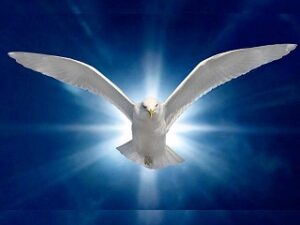
\includegraphics[width=.3\textwidth]{holy-spirit-dove_SI-300x225.jpg}
\end{wrapfigure}

Holy Spirit becomes present after the 40 days of secret teachings to the disciples. The vertical dimension of the Spirit is outside history so that esoteric teaching is ahistorical and contends with dogmatic teaching, which is historical. The Hermetic teaching preserves the esoteric teaching, but has no pretense to create a new religion. \textbf{Valentin Tomberg} writes in the \emph{Meditations on the Tarot}:


\begin{quotex}
They do not secretly guard a religion, which to them is appropriate, to replace the existing religions, or a science to replace the current sciences, or arts to replace the fine arts of today or yesterday. That which they possess does not comprise any tangible advantage or objective superiority with regard to religion, science and art; what they possess is only the communal soul of religion, science and art.
\end{quotex}


Hermeticism, therefore, is outside history and is therefore not an alternative to philosophy, religion, science, or art. He goes on:

\begin{quotex}
Hermeticism, the living Hermetic tradition, guards the communal soul of all true culture. I must add: Hermeticists listen to --- and now and then hear---the beating of the heart of the spiritual life of humanity. They cannot do otherwise than live as guardians of the life and communal soul of religion, science and art. They do not have any privilege in any of these domains; saints, true scientists, and artists of genius are their superiors. But they live for the mystery of the communal heart which beats within all religions, all philosophies, all arts and all sciences --- past, present and future.
\end{quotex}


Tomberg then refers to humanity as an organism: ``Hermeticism is a ``ferment'' or an ``enzyme'' in the organism of the spiritual life of humanity.'' That refers to Great Being, the Eternal Sophia, described by \textbf{Vladimir Solovyov}.


\paragraph{Fedeli d'Amore}


The Iranian mystic Ruzbehan distinguishes between the pious ascetics who never experienced human love and the \emph{Fedeli d'Amore}, for whom the experience of a cult of love dedicated to a beautiful woman is the necessary initiation to divine love, from which it is inseparable.

For Ibn Arabi, it was Nizam, and for Dante, Beatrice. They thus fall outside the system of the chain of initiations. Ibn Arabi was initiated directly by Khidr. Khidr is outside time, appearing in different eras as a different figure.

The beautiful beings beloved by Ibn Arabi and Dante transfigure human \emph{eros}; she becomes for each of them a theophany of Divine Love.


\paragraph{The End of a World}


Man needs a buffer, like an automobile shock absorber, to protect him from the shocks of life. This he does by lying. Lies turn everything into its opposite, so that the real world is obscured by a web of lies. He even lies about lying so he never has to question the factitious world he created. The Vedic teachings warn against this artificial superstructure created atop reality.

Inspiration comes when the lies stop and reality is seen for what it is. The end of a world is the end of an illusion.

\url{https://www.youtube.com/watch?v=nXzTre7ujEw} 

\flrightit{Posted on 2022-06-05 by Cologero}

\begin{center}* * *\end{center}

\begin{footnotesize}
\begin{sffamily}
\texttt{Balder on 2022-06-09 at 13:35 said:}

In easter Sunday evening while going asleep I saw a white dove descend upon my head. I took it as a sign of inspiration from above. Now I've become very careful not to spoil the treasures I've been given. Tomberg has been very inspirational.

\hfill

\texttt{Balder on 2022-06-09 at 16:51 said:}

I've come to the conclusion that we're too good for this world.

\url{https://biblehub.com/nlt/hebrews/11-38.htm}


\hfill

\texttt{Max on 2022-06-20 at 08:54 said:}

``The vertical dimension of the Spirit is outside history so that esoteric teaching is ahistorical''

Initiates ``thus fall outside the system of the chain of initiations.''

Initiation trough a chain of initiation is like coming to know the ahistorical through history. It belongs to the type of things which is written about in history books. Even the bible is but a history book in the opinion of the believers. Therefore the chain of initiation is but the tradition of contending with the dogmas of history, or at least so it seems to history.

\end{sffamily}
\end{footnotesize}

